\chapter{Semantics-First Approach to Clinical Decision Support}

In chapter \ref{chapter:introduction}, we explained that, despite
advances in medicine, mortality and costs associated with preventable
medical errors (\PMEs{}) remain unacceptably high. In chapter
\ref{chapter:background}, we explained how systems that
assist healthcare practitioners (\HCPs{}) with situation-specific
advice based on evidence-based best practice guidelines (\BPGs{}),
called clinical decision (\CDSSs{}) can reduce both mortality
and costs associated with \PMEs{}. But, despite their potential,
the uptake of such systems in practice is hindered by challenges
that were introduced in section \ref{sec:hurdles-cdss-adoption}, and
discussed in depth in chapter \ref{chapter:hurdles-cdss-adoption}.
In brief, the following challenges (Cs) were outlined:
\begin{enumerate}[label=C\arabic*.]
\itemsep0.0em
\item Absence of systematic ways of \emph{validating content}
in a \emph{reliable}, \emph{accessible} and \emph{updateable} manner.
\item Lack of \emph{reliable}, \emph{shareable} \CDSS{} content
that can be easily adopted across healthcare organizations and their (Information
Technology) \IT{} systems.
\item Technical difficulties of sharing due to \emph{need for
  adaptation} to diverse Electronic Health Records (\EHR) systems.
\item \emph{Suboptimal} User Interfaces (\UIs), implementation choices and
workflows.
\end{enumerate}

\begin{figure}[bh]
  \centering
  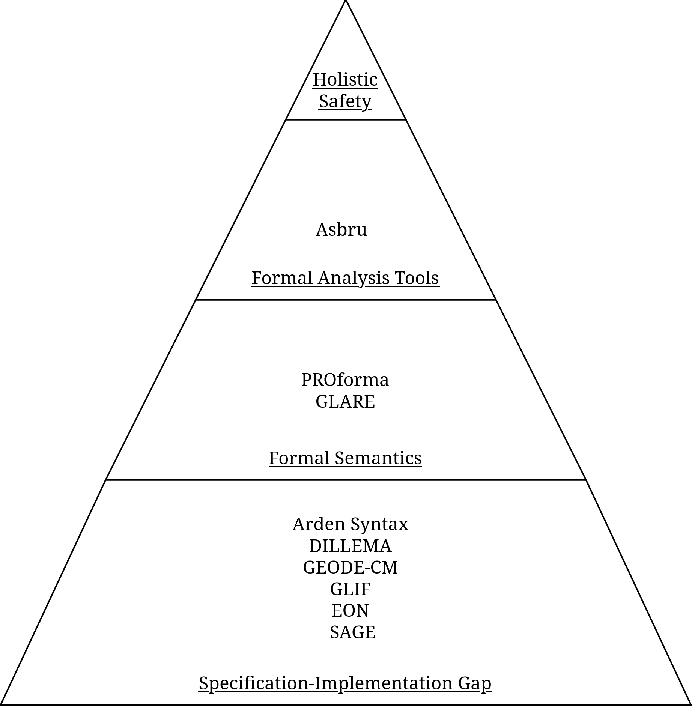
\includegraphics[width=0.4\textwidth]{pyramid}
  \caption{Existing \DSLs{} for Computer Interpretable Guidelines}\label{fig:existing-work-pyramid}
\end{figure}

Over the years, significant progress has been made towards
addressing these challenges. In chapter \ref{chapter:related-work},
we discussed how existing approaches have attempted to
address said challenges, and their limitations. Specifically,
in section \ref{sec:related-work-discussion}, we outlined major
themes that these approaches adopt to tackle these challenges.
This is further illustrated by the pyramid diagram in \figurename{}
\ref{fig:existing-work-pyramid}, where aforementioned themes are
underlined in the pyramid's various rungs.
As is typical, approaches that appear in higher rungs also
have characteristics of ones below them. For example, while guidelines expressed in
the Arden Syntax eliminate the specification-implementation gap by being
both \HCP{}-comprehensible and interpretable, they cannot be formally analyzed
due to lack of analysis tools in the ecosystem. Asbru-based guidelines
on the other hand not only eliminate the specification-implementation gap, but can also be
formally analyzed using support for KIV-based verification in the Asbru
ecosystem (see section \ref{sec:kiv-verification}).

As is evident in \figurename{} \ref{fig:existing-work-pyramid}



